
\lstdefinelanguage{plaintext}{
  sensitive=false,
  comment=[l]{//},
  morecomment=[s]{/*}{*/},
  identifierstyle=\color{black},
  morestring=[b]',
  morestring=[b]"
}

\lstset
{ 
    language=plaintext,
    basicstyle=\footnotesize,
    numbers=left,
    stepnumber=1,
    showstringspaces=false,
    tabsize=1,
    breaklines=true,
    breakatwhitespace=false,
    frame=leftline
}

\chapter{Implementasi dan Pengujian}
\label{chap:implementasidanpengujian}
Pada bab dijelaskan mengenai implementasi perangkat lunak dan pengujian perangkat lunak. Bagian implementasi berisi tentang lingkungan implementasi dan hasil implementasi. Bagian pengujian berisi tentang pengujian fungsional dan pengujian eksperimental. 

\section{Implementasi}
\label{sec:implementasi}
\subsection{Lingkungan Implementasi}
\label{subsec:lingkunganimplementasi5}
Implementasi dari perangkat lunak dilakukan pada sebuah laptop. Berikut adalah spesifikasi laptop dan perangkat lunak yang digunakan untuk prapengujian:
\begin{itemize}
\item Processor: Intel Core i3 4030U
\item RAM: 6GB
\item Sistem Operasi: Windows 10 pro 64-bit
\item Versi Apache HTTP Server: 2.4.29
\item Versi MySQL Server: 5.5.5
\item Versi Netbeans: 8.1
\item Versi Google Chrome: 73.0.3683.86
\end{itemize}

\subsection{Hasil Implementasi}
\label{subsec:lingkunganimplementasi}
Hasil dari implementasi adalah sebuah perangkat berbasis terminal yang dapat membangkitkan animasi \textit{timelapse} pada pengembangan proyek perangkat lunak berbasis \textit{web}. Kode program dari perangkat lunak dapat dilihat pada Lampiran \ref{lamp:A}. Setelah dijalankan, perangkat lunak akan menghasilkan dua \textit{output} yaitu, status pada terminal dan \textit{file} hasil animasi bertipe GIF.
\begin{enumerate}
\item \textbf{Status pada Terminal}\\
Setelah berhasil membangkitkan animasi \textit{timelapse}, perangkat lunak menampilkan status pada terminal seperti yang diperlihatkan pada Listing \ref{lst:status_berhasil}. Baris 5 menunjukkan bahwa animasi \textit{timelapse} berhasil dibangkitkan. Pesan pada baris 1-4 muncul saat ChromeDriver membuka dan mulai mengontrol Chrome \textit{browser}.

\begin{lstlisting}[caption={Status pesan pada terminal saat program berhasil membangkitkan animasi \textit{timelapse}.},label={lst:status_berhasil},language=plaintext]
Starting ChromeDriver 2.42.591088 (7b2b2dca23cca0862f674758c9a3933e685c27d5) on port 16446
Only local connections are allowed.
Feb 24, 2019 3:26:25 PM org.openqa.selenium.remote.ProtocolHandshake createSession
INFO: Detected dialect: OSS
Animasi timelapse berhasil dibuat
\end{lstlisting}

\item \textbf{\textit{File} GIF Hasil Animasi}\\
Selain menghasilkan status pada terminal, program juga akan menghasilkan sebuah \textit{file} GIF hasil animasi.
Gambar \ref{fig:c1} menunjukkan \textit{screenshot} setiap \textit{commit} yang terdapat pada \textit{file} GIF hasil animasi dari proyek Piktora. Piktora memiliki 58 \textit{commit}, sehingga terdapat 58 \textit{screenshot}. 


\begin{figure}[H]
	
		\includegraphics[scale=0.3]{Gambar/Piktora.png}
	\caption{\textit{Screenshot} proyek Piktora pada \textit{commit} 315d374 (31 Oktober 2016) - \textit{commit} 89000be (12 Januari 2018).}
	\label{fig:c1}
\end{figure}





\end{enumerate}
\section{Pengujian}
\label{sec:pengujian}

\subsection{Pengujian Fungsional}
\label{sec:pengujian_fungsional} 
Pengujian ini dilakukan dengan tujuan untuk mengetahui apakah Command Line Option yang terdapat pada program sudah berjalan dengan baik. \textit{Option} yang terdapat pada program dapat dilihat pada subbab \ref{sec:analisis_fitur_aplikasi}. Lingkungan pengujian fungsional sama dengan lingkungan implementasi yang terdapat pada subbab \ref{subsec:lingkunganimplementasi5}. Pengujian dilakukan pada proyek Piktora dengan menggunakan berbagai macam tes kasus. Histori \textit{commit} proyek Piktora dapat dilihat pada subbab \ref{sec:prapengujian}. Hasil pengujian fungsional dapat dilihat pada Tabel \ref{table:hasil_pengujian1} sampai dengan Tabel \ref{table:hasil_pengujian3}.


\begin{table}[htbp]
	\centering
	\caption{Tabel pengujian fungsional}
	
		\begin{tabular}{|p{0.3cm}|>{\raggedright} p{5.5 cm}| p{7 cm}| p{3 cm}|} \hline
		No & Tes Kasus	& \texttt{Output} yang diharapkan & \textit{Output} program \\ \hline
		1. & Menguji \textit{option} \texttt{-project-path} menggunakan path yang valid. Argumen Command Line yang diberikan ke program: \texttt{-project-path C:/xampp/htdocs/Piktora/.git} & Program berhasil membangkitkan animasi berdasarkan path yang diberikan dan mengeluarkan status pesan "Animasi timelapse berhasil dibuat" & sesuai \\ \hline
		2. & Menguji \textit{option} \texttt{-project-path} menggunakan path yang tidak valid. Argumen Command Line yang diberikan ke program: \texttt{-project-path C:/xampp/htdocs}  & Program gagal membuat animasi dan mengeluarkan pesan error "Path proyek tidak valid"  & sesuai \\ \hline
		3. & Menguji \textit{option} \texttt{-capture-url} menggunakan satu argumen. Argumen Command Line yang diberikan ke program:  \texttt{-capture-url http://localhost} & Program mengambil screenshot berdasarkan alamat yang diberikan. Tampilan dari \textit{file} hasil animasi dapat dilihat pada Gambar \ref{fig:capture1}  & sesuai	\\ \hline
		4. & Menguji \textit{option} \texttt{-capture-url} menggunakan dua argumen. Argumen Command Line yang diberikan ke program:  \texttt{-capture-url http://localhost http://localhost/about} & Program mengambil screenshot berdasarkan alamat-alamat yang diberikan. Tampilan dari \textit{file} hasil animasi dapat dilihat pada Gambar \ref{fig:capture2}  & sesuai \\ \hline
		5. & Menguji \textit{option} \texttt{-capture-url} menggunakan tiga argumen. Argumen Command Line yang diberikan ke program:  \texttt{-capture-url http://localhost http://localhost/about http://localhost/projects} & Program mengambil screenshot berdasarkan alamat-alamat yang diberikan. Tampilan dari \textit{file} hasil animasi dapat dilihat pada Gambar \ref{fig:capture3}   & sesuai\\ \hline
		6. & Menguji \textit{option} \texttt{-capture-url} menggunakan empat argumen. Argumen Command Line yang diberikan ke program:  \texttt{-capture-url http://localhost http://localhost/about http://localhost/projects http://localhost/contact} & Program mengambil screenshot berdasarkan alamat-alamat yang diberikan. Tampilan dari \textit{file} hasil animasi dapat dilihat pada Gambar \ref{fig:capture4}  & sesuai \\ \hline
		7. & Menguji \textit{option} \texttt{-capture-url} menggunakan lima argumen. Argumen Command Line yang diberikan ke program:  \texttt{-capture-url http://localhost http://localhost/about http://localhost/projects http://localhost/contact http://localhost/projects/1}& Program gagal membuat animasi dan mengeluarkan pesan error "Jumlah url yang akan dicapture maksimal 4" & sesuai \\ \hline
		
		
		
		
		\end{tabular}
	\label{table:hasil_pengujian1}
\end{table}


\begin{table}[htbp]
	\centering
	\caption{Tabel pengujian fungsional}
	
		\begin{tabular}{|p{0.3cm}|>{\raggedright} p{7 cm}| p{5.5 cm}| p{3 cm}|} \hline
		No & Tes Kasus	& \textit{Output} yang diharapkan & \textit{Output} program \\ \hline
		8. & Menguji \textit{option} \texttt{-seconds-per-commit} dengan nilai 2. Argumen Command Line yang diberikan ke program: \texttt{-seconds-per-commit 2} & Program berhasil membangkitkan animasi dan menghasilkan \textit{file} GIF yang memiliki durasi 116 detik & sesuai \\ \hline
		9. & Menguji \textit{option} \texttt{-seconds-per-commit} dengan nilai 0. Argumen Command Line yang diberikan ke program: \texttt{-seconds-per-commit 0} & Program gagal membuat animasi dan mengeluarkan pesan error "Seconds per commit harus lebih besar dari 0" & sesuai \\ \hline
		10. & Menguji \textit{option} \texttt{-seconds-per-commit} dengan nilai 656. Argumen Command Line yang diberikan ke program: \texttt{-seconds-per-commit 656} & Program gagal membuat animasi dan mengeluarkan pesan error "Seconds per commit harus kurang dari sama dengan  655" & sesuai \\ \hline
		11. & Menguji \textit{option} \texttt{-before-capture}. Argumen Command Line yang diberikan ke program: \texttt{-before-capture "php script\_piktora.php"} & Program menjalankan \textit{terminal command} sebelum mengambil \textit{screenshot} & sesuai  \\ \hline
		
		12. & Menguji \textit{option} \texttt{-title}. Argumen Command Line yang diberikan ke program: \texttt{-title Piktora}  & Program berhasil membangkitkan animasi dan menghasilkan \textit{file} GIF, dimana di dalam \textit{file} tersebut terdapat judul yang terletak di pojok kiri bawah(lihat Gambar \ref{fig:title}). & sesuai \\ \hline
					
		13. & Menguji \textit{option} \texttt{-logo} menggunakan \textit{path} gambar yang valid. Argumen Command Line yang diberikan ke program: \texttt{-logo Logo-UNPAR.png} & Program berhasil membangkitkan animasi dan menghasilkan \textit{file} GIF, dimana di dalam \textit{file} tersebut logo yang terletak di pojok kanan bawah (lihat Gambar \ref{fig:logo}) & sesuai  \\ \hline
		14. & Menguji \textit{option} \texttt{-logo} menggunakan \textit{path} gambar yang tidak valid. Argumen Command Line yang diberikan ke program: \texttt{-logo script\_piktora.php} & Program gagal membuat animasi dan mengeluarkan pesan error "Path gambar tidak valid" & sesuai  \\ \hline
		15. & Menguji \textit{option} \texttt{-branch} menggunakan \textit{branch} yang valid. Argumen Command Line yang diberikan ke program: \texttt{-branch master} & Program membangkitkan animasi pada \textit{branch} master & sesuai  \\ \hline
		16. & Menguji \textit{option} \texttt{-branch} menggunakan \textit{branch} yang tidak valid. Argumen Command Line yang diberikan ke program: \texttt{-branch piktora}  & Program gagal membuat animasi dan mengeluarkan pesan error "Branch tidak valid" & sesuai  \\ \hline
		17. & Menguji \textit{option} \texttt{-start-commit} menggunakan \textit{commit} ID dengan panjang 7 karakter. Argumen Command Line yang diberikan ke program:  \texttt{-start-commit 9b0a302} & Program membangkitkan animasi dimulai dari commit 9b0a302 & sesuai  \\ \hline		
		
		
\end{tabular}
	\label{table:hasil_pengujian2}
\end{table}


\begin{table}[htbp]
	\centering
	\caption{Tabel pengujian fungsional}
	
		\begin{tabular}{|p{0.3cm}|>{\raggedright} p{7 cm}| p{5.5 cm}| p{3 cm}|} \hline
		No & Tes Kasus	& \textit{Output} yang diharapkan & \textit{Output} program \\ \hline

18. & Menguji \textit{option} \texttt{-start-commit} menggunakan \textit{commit} ID dengan panjang kurang dari 7 karakter. Argumen Command Line yang diberikan ke program: \texttt{-start-commit 9b0a30} & Program gagal membuat animasi dan mengeluarkan pesan error "Panjang commit ID awal harus berada di antara 7-40 karakter" & sesuai  \\ \hline
		19.&  Menguji \textit{option} \texttt{-start-commit} menggunakan \textit{commit} ID dengan panjang lebih dari 40 karakter. Argumen Command Line yang diberikan ke program:  \texttt{-start-commit 9b0a3023ac8c94c67f4c1b39388277768a4 83dba9} & Program gagal membuat animasi dan mengeluarkan pesan error "Panjang commit ID awal harus berada di antara 7-40 karakter" & sesuai  \\ \hline
		20. & Menguji \textit{option} \texttt{-stop-commit} menggunakan \textit{commit} ID dengan panjang 7 karakter. Argumen Command Line yang diberikan ke program:  \texttt{-stop-commit 6a085c1}  & Program membangkitkan animasi dimulai dari \textit{commit} 315d374 sampai dengan \textit{commit 6a085c1}  & sesuai  \\ \hline
		21. & Menguji \textit{option} \texttt{-stop-commit} menggunakan \textit{commit} ID dengan panjang kurang dari 7 karakter. Argumen Command Line yang diberikan ke program: \texttt{-stop-commit 6a085c} & Program gagal membuat animasi dan mengeluarkan pesan error "Panjang commit ID akhir harus berada di antara 7-40 karakter" & sesuai  \\ \hline
		22. & Menguji \textit{option} \texttt{-stop-commit} menggunakan \textit{commit} ID dengan panjang lebih dari 40 karakter. Argumen Command Line yang diberikan ke program: \texttt{-stop-commit 6a085c1c37949e6308cfe06a117302e5283 88e549} & Program gagal membuat animasi dan mengeluarkan pesan error "Panjang commit ID akhir harus berada di antara 7-40 karakter"  & sesuai  \\ \hline
		23. & Menguji \textit{option} \texttt{-start-commit} dan \textit{option} \texttt{-stop-commit} menggunakan rentang \textit{commit} yang valid. Argumen Command Line yang diberikan ke program: \texttt{-start-commit 9b0a302 -stop-commit 6a085c1} & Program membangkitkan animasi dimulai dari \textit{commit} 9b0a302 sampai dengan \textit{commit} 6a085c1 & sesuai  \\ \hline
		24. & Menguji \textit{option} \texttt{-start-commit} dan \textit{option} \texttt{-stop-commit} menggunakan rentang \textit{commit} yang tidak valid. Argumen Command Line yang diberikan ke program: \texttt{-start-commit 6a085c1 -stop-commit 9b0a302} & Program gagal membuat animasi dan mengeluarkan pesan error "Commit ID awal dan akhir terbalik"  & sesuai\\ \hline
		25. & Menguji \textit{option} \texttt{-start-commit} dan \textit{option} \texttt{-stop-commit} menggunakan rentang \textit{commit} yang tidak valid. Argumen Command Line yang diberikan ke program: \texttt{-start-commit 9b0a302  -stop-commit 9b0a302} & Program gagal membuat animasi dan mengeluarkan pesan error "Commit ID awal dan akhir tidak boleh sama" & sesuai  \\ \hline
\end{tabular}
	\label{table:hasil_pengujian3}
\end{table}


\ \\
\ \\
\begin{figure}[H]
	\centering
		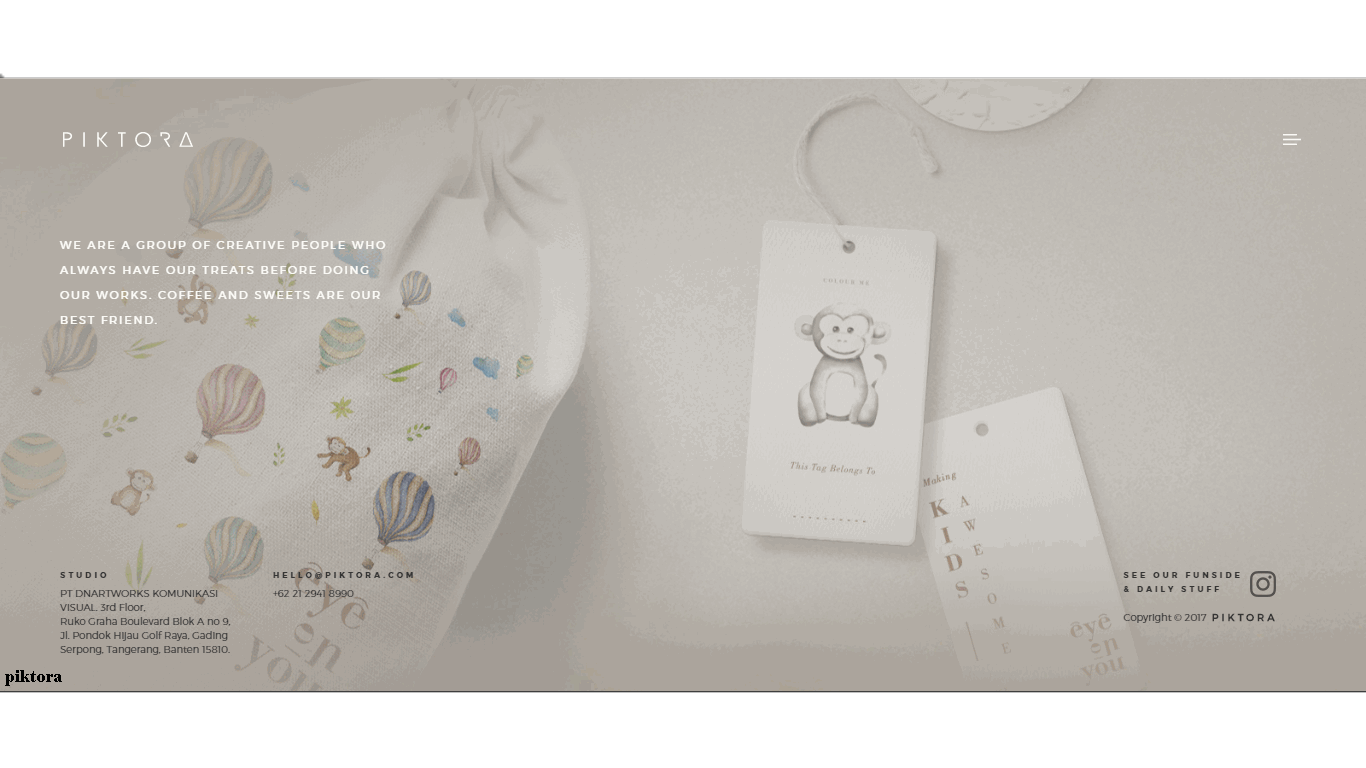
\includegraphics[scale=0.3]{Gambar/title.png}
	\caption{Salah satu \textit{commit} yang terdapat pada \textit{file} hasil animasi. Terdapat judul dibagian pojok kiri bawah.}
	\label{fig:title}
\end{figure}


\begin{figure}[H]
	\centering
		
\includegraphics[scale=0.3]{Gambar/logo.png}
	\caption{Salah satu \textit{commit} yang terdapat pada \textit{file} hasil animasi. Terdapat logo dibagian pojok kanan bawah.}
	\label{fig:logo}
\end{figure}

\begin{figure}[H]
	\centering
		
\includegraphics[scale=0.3]{Gambar/capture1.png}
	\caption{Salah satu \textit{commit} pada \textit{file} hasil animasi jika terdapat satu argumen \texttt{-capture-url}.}
	\label{fig:capture1}
\end{figure}



\begin{figure}[H]
	\centering
		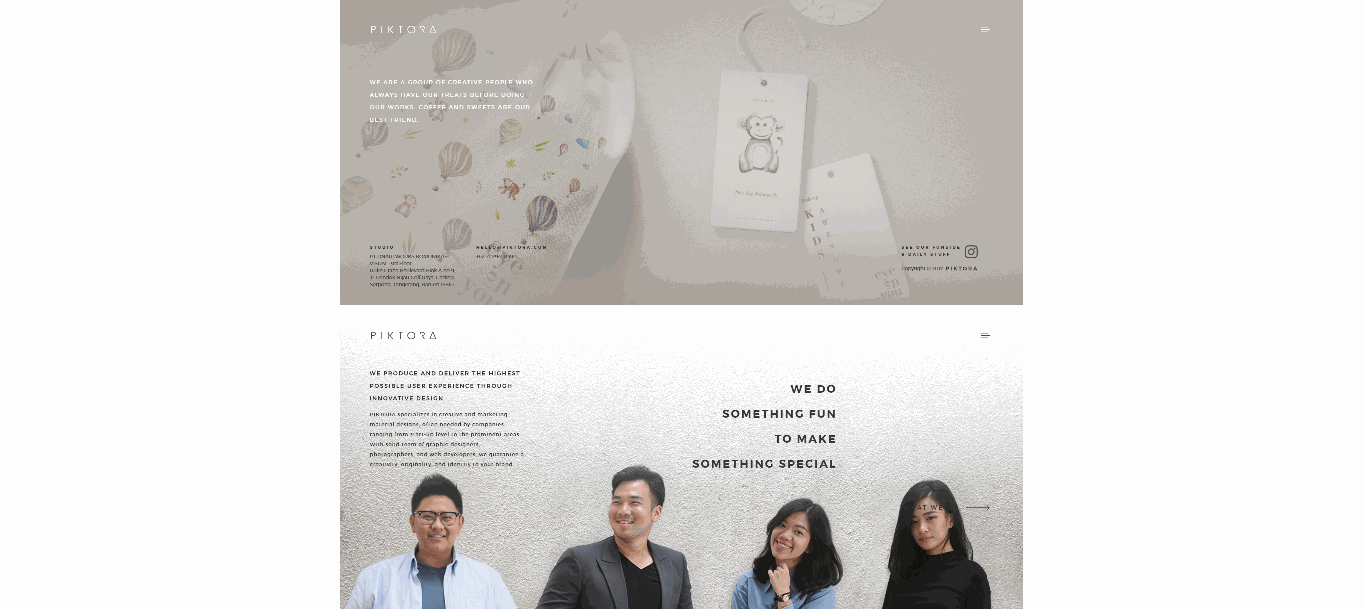
\includegraphics[scale=0.3]{Gambar/capture2.png}
	\caption{Salah satu \textit{commit} pada \textit{file} hasil animasi jika terdapat dua argumen \texttt{-capture-url}.}
	\label{fig:capture2}
\end{figure}



\begin{figure}[H]
	\centering
		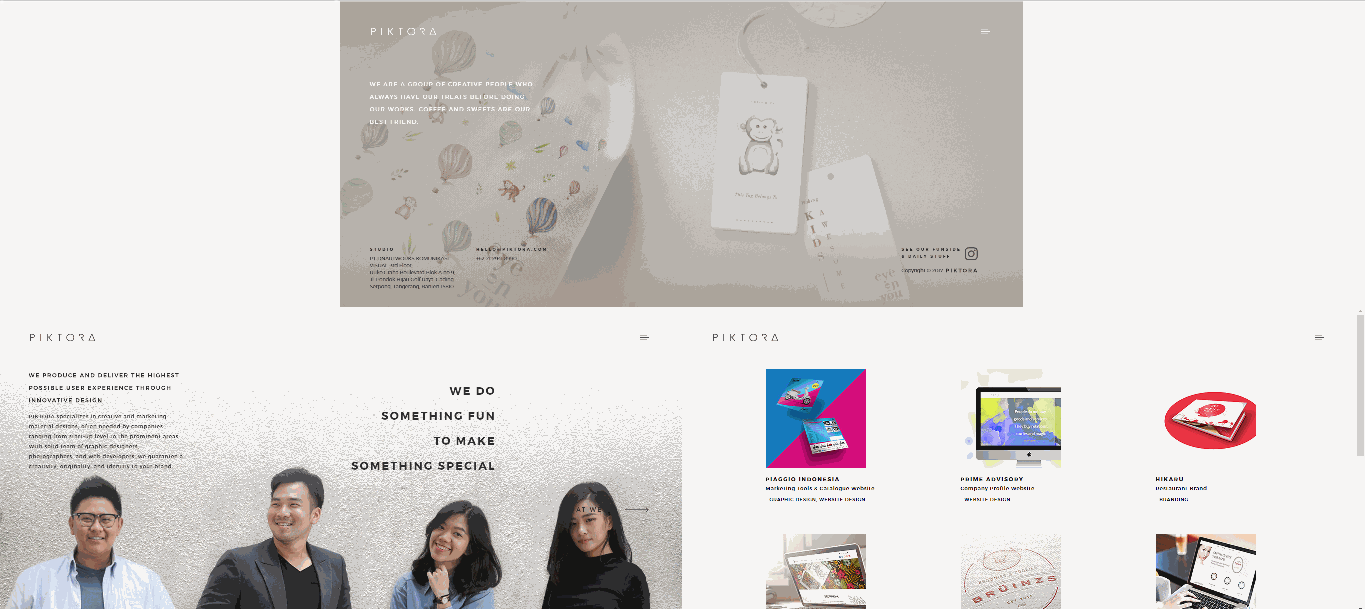
\includegraphics[scale=0.3]{Gambar/capture3.png}
	\caption{Salah satu \textit{commit} pada \textit{file} hasil animasi jika terdapat tiga argumen \texttt{-capture-url}.}
	\label{fig:capture3}
\end{figure}


\begin{figure}[H]
	\centering
		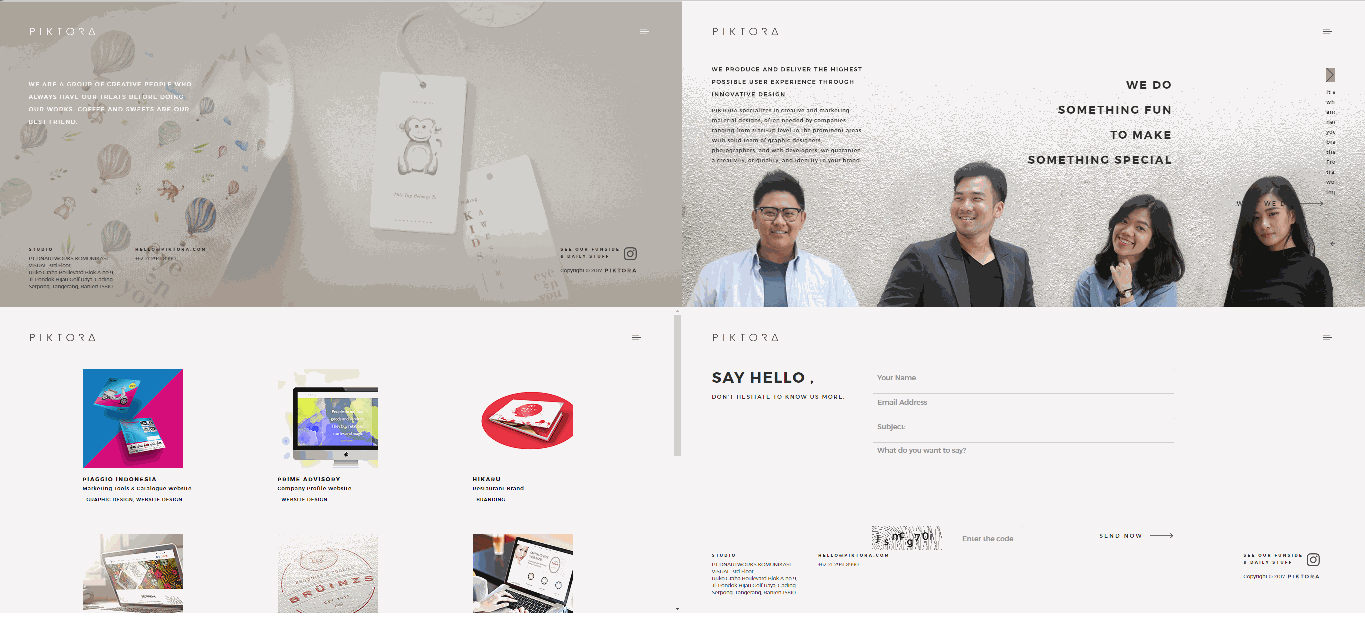
\includegraphics[scale=0.3]{Gambar/capture4.png}
	\caption{Salah satu \textit{commit} pada \textit{file} hasil animasi jika terdapat empat argumen \texttt{-capture-url}.}
	\label{fig:capture4}
\end{figure}




\subsection{Pengujian Eksperimental}
\label{sec:pengujian_eksperimental} 
Pengujian eksperimental ini dibagi menjadi dua bagian. Pengujian eksperimental bagian pertama akan menguji program menggunakan proyek Piktora dengan WebDriver yang berbeda. WebDriver yang digunakan untuk pengujian ini yaitu FirefoxDriver, EdgeDriver, OperaDriver, dan InternetExplorerDriver. Pengujian eksperimental bagian kedua akan menguji progam dengan situs \texttt{web} Bootstrap\footnote{https://getbootstrap.com/}, Netflix Open Source Software Center\footnote{https://netflix.github.io/}, IBM Open Source\footnote{https://ibm.github.io/}, React\footnote{https://reactjs.org/}, dan Yelp Open Source\footnote{https://yelp.github.io/}. 

Seperti yang sudah dijelaskan pada subbab \ref{sec:selenium_webdriver} FirefoxDriver, EdgeDriver, OperaDriver, dan InternetExplorerDriver merupakan implementasi dari WebDriver yang mengontrol \textit{browser} yang mengontrol \textit{browser} tertentu. FirefoxDriver mengontrol Firefox \textit{browser}, OperaDriver mengontrol Opera \textit{browser}, dst. Tujuan dari digunakannya berbagai macam WebDriver ini adalah untuk menguji program dalam membangkitkan animasi menggunakan berbagai macam \textit{browser}.

Pengujian kedua ini dilakukan dengan tujuan menguji program dengan berbagai situs \textit{web} yang berbeda dan memiliki jumlah \textit{commit} yang berbeda. Situs \textit{web} Bootstrap, Netflix Open Source Software Center, IBM Open Source, React, dan Yelp Open Source  dipilih karena bersifat Open Source, repositorinya tersimpan pada GitHub, dan dihosting menggunakan GitHub Pages. GitHub Pages\footnote{https://pages.github.com/} merupakan sebuah layanan \textit{hosting} situs \textit{web} untuk melakukan \textit{hosting} halaman \textit{web} secara langsung dari repositori GitHub.     

Berikut adalah rincian dari pengujian eksperimental:

\begin{enumerate}
\item \textbf{Pengujian Proyek Piktora dengan FirefoxDriver}\\
Pengujian pada proyek Piktora dilakukan menggunakan FirefoxDriver. Pada saat melakukan pengujian, kode program pada kelas BrowserController baris ke-46  diubah (lihat Lampiran \ref{lamp:A}). \textit{Object} bertipe WebDriver dinisialisasi menggunakan \textit{object} bertipe FirefoxDriver. Versi Firefox \textit{browser} yang digunakan untuk pengujian adalah 66.0.2. Gambar \ref{fig:firefox}, menunjukkan tampilan Firefox \textit{browser} saat dikontrol oleh FirefoxDriver. Berikut ini adalah \textit{option} yang digunakan untuk menguji program:
\begin{itemize}
\item \texttt{-project-path C:/xampp/htdocs/Piktora/.git}
\item \texttt{-capture-url http://localhost}
\item \texttt{-before-capture "php script\_piktora.php"}
\end{itemize}
Program berhasil membangkitkan animasi \textit{timelapse} pada proyek Piktora menggunakan FirefoxDriver.

\begin{figure}[H]
	\centering
		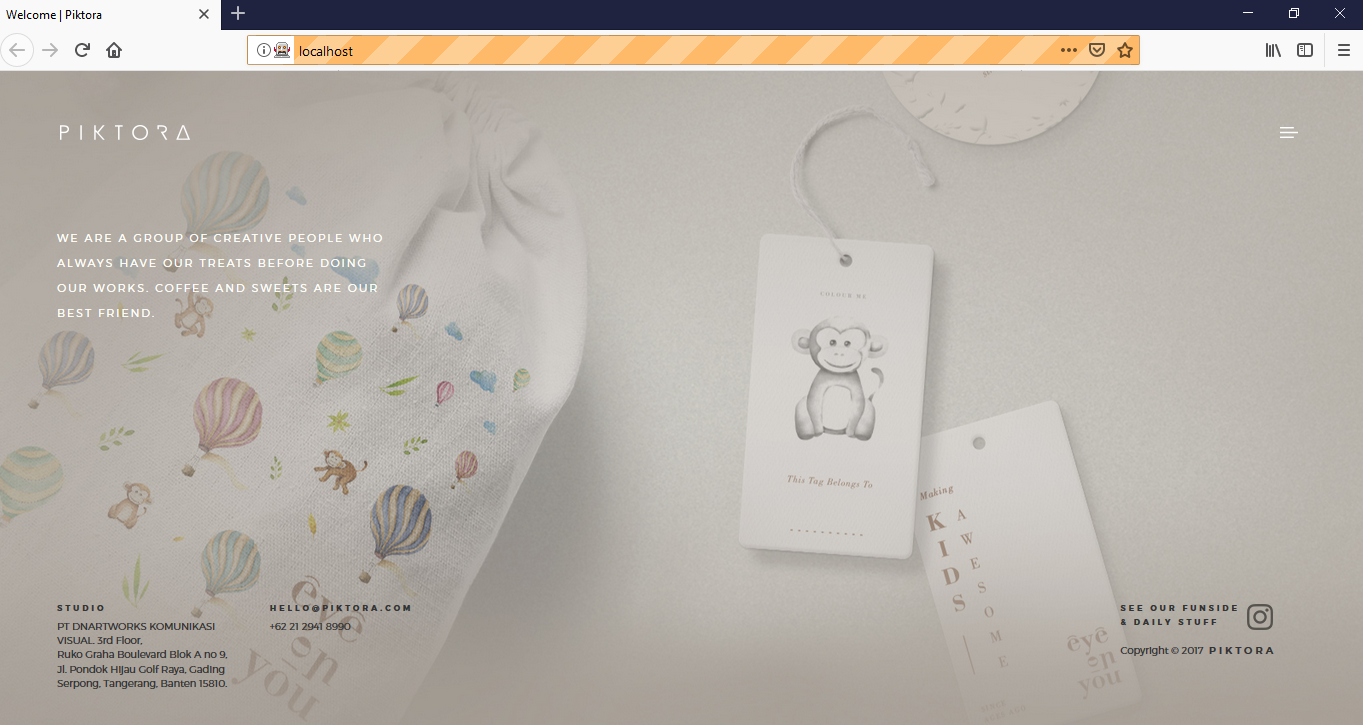
\includegraphics[scale=0.4]{Gambar/Firefox.png}
	\caption{Tampilan pada Firefox \textit{browser} saat dikontrol oleh FirefoxDriver.}
	\label{fig:firefox}
\end{figure}




\item \textbf{Pengujian Proyek Piktora dengan OperaDriver}\\
Pengujian pada proyek Piktora dilakukan menggunakan OperaDriver. Pada saat melakukan pengujian, kode program pada kelas BrowserController baris ke-46  diubah (lihat Lampiran \ref{lamp:A}). \textit{Object} bertipe WebDriver dinisialisasi menggunakan \textit{object} bertipe OperaDriver. Versi Opera \textit{browser} yang digunakan untuk pengujian adalah 60.0.3255.27 (portable version). Gambar \ref{fig:opera} menunjukkan tampilan pada Opera \textit{browser} saat dikontrol oleh OperaDriver. Berikut ini adalah \textit{option} yang digunakan untuk menguji program:
\begin{itemize}
\item \texttt{-project-path C:/xampp/htdocs/Piktora/.git}
\item \texttt{-capture-url http://localhost}
\item \texttt{-before-capture "php script\_piktora.php"}
\end{itemize}

Terdapat masalah saat melakukan pengujian. Awalnya Opera \textit{browser} yang digunakan bukan versi \textit{portable} melainkan versi standar. Saat program dijalankan, program mengeluarkan pesan \textit{error} berupa \texttt{unknown error: cannot find Opera binary}. Setelah ditelusuri, tidak ditemukan \textit{file} "opera.exe" di dalam direktori "C:/Program Files" atau "C:/Program Files (x86)". Solusi untuk mengatasi masalah ini adalah melakukan instalasi Opera \textit{browser} versi \textit{portable} pada direktori "C:/Program Files" atau "C:/Program Files (x86)". Setelah dilakukan instalasi tersebut, program berhasil membangkitkan animasi \textit{timelapse} pada proyek Piktora menggunakan OperaDriver. 

\begin{figure}[H]
	\centering
		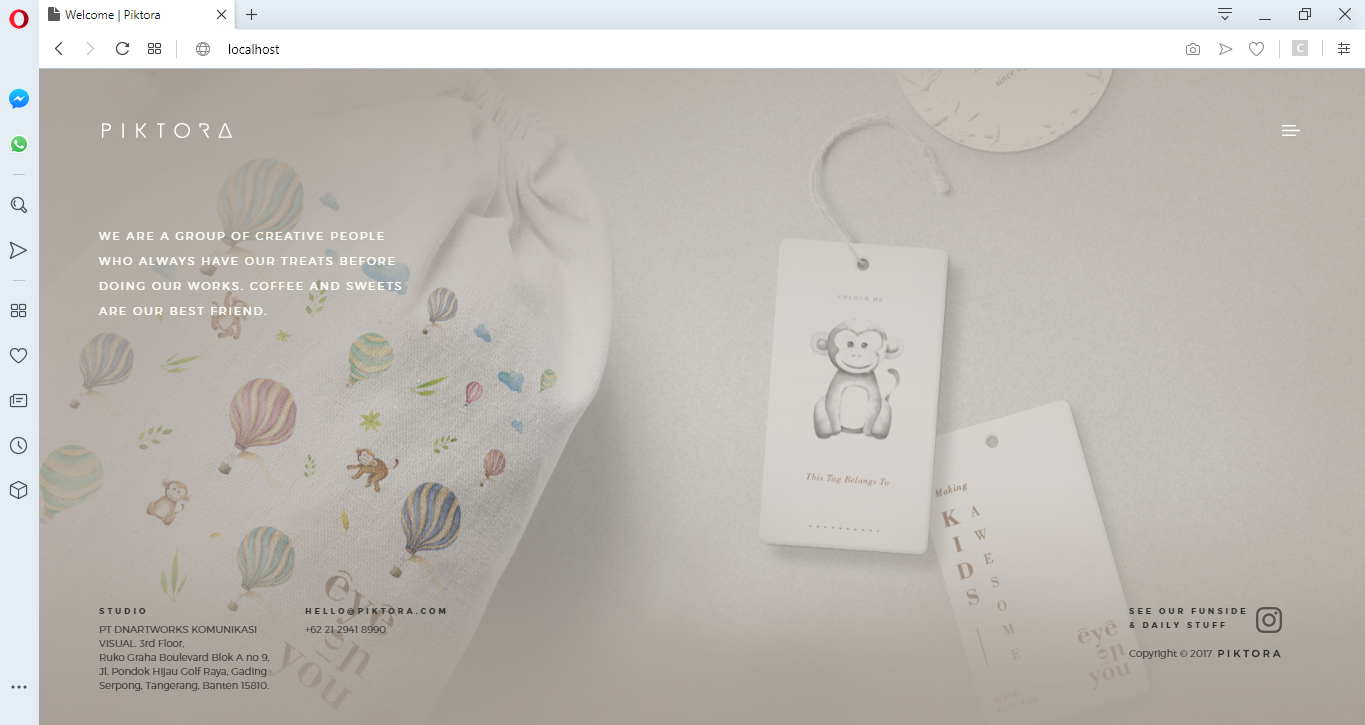
\includegraphics[scale=0.4]{Gambar/Opera.png}
	\caption{Tampilan pada Opera \textit{browser} saat dikontrol oleh OperaDriver.}
	\label{fig:opera}
\end{figure}


\item \textbf{Pengujian Proyek Piktora dengan EdgeDriver}\\
Pengujian pada proyek Piktora dilakukan menggunakan EdgeDriver. Pada saat melakukan pengujian, kode program pada kelas BrowserController baris ke-46  diubah (lihat Lampiran \ref{lamp:A}). \textit{Object} bertipe WebDriver dinisialisasi menggunakan \textit{object} bertipe EdgeDriver. Versi Microsoft Edge \textit{browser} yang digunakan untuk pengujian adalah 44.17763.1.0. Berikut ini adalah \textit{option} yang digunakan untuk menguji program:
\begin{itemize}
\item \texttt{-project-path C:/xampp/htdocs/Piktora/.git}
\item \texttt{-capture-url http://localhost}
\item \texttt{-before-capture "php script\_piktora.php"}
\end{itemize}
Hasil pengujian ini tidak sesuai dengan harapan. Tampilan halaman \textit{web} yang ditampilkan oleh Microsoft Edge \textit{browser} saat dikontrol oleh EdgeDriver tidak rapih seperti yang diperlihatkan pada Gambar \ref{fig:layout1}. Tidak diketahui apa yang menyebabkan halaman \textit{web} tersebut menjadi tidak rapih. Sebagai perbandingan, Gambar \ref{fig:layout2} menunjukkan tampilan halaman \textit{web} yang ditampilkan oleh Microsoft Edge \textit{browser} saat tidak dikontrol oleh EdgeDriver. Meskipun tampilan dari halaman \textit{web} tidak rapih, program tetap dapat membangkitkan animasi pada proyek Piktora.    

\begin{figure}[H]
	\centering
		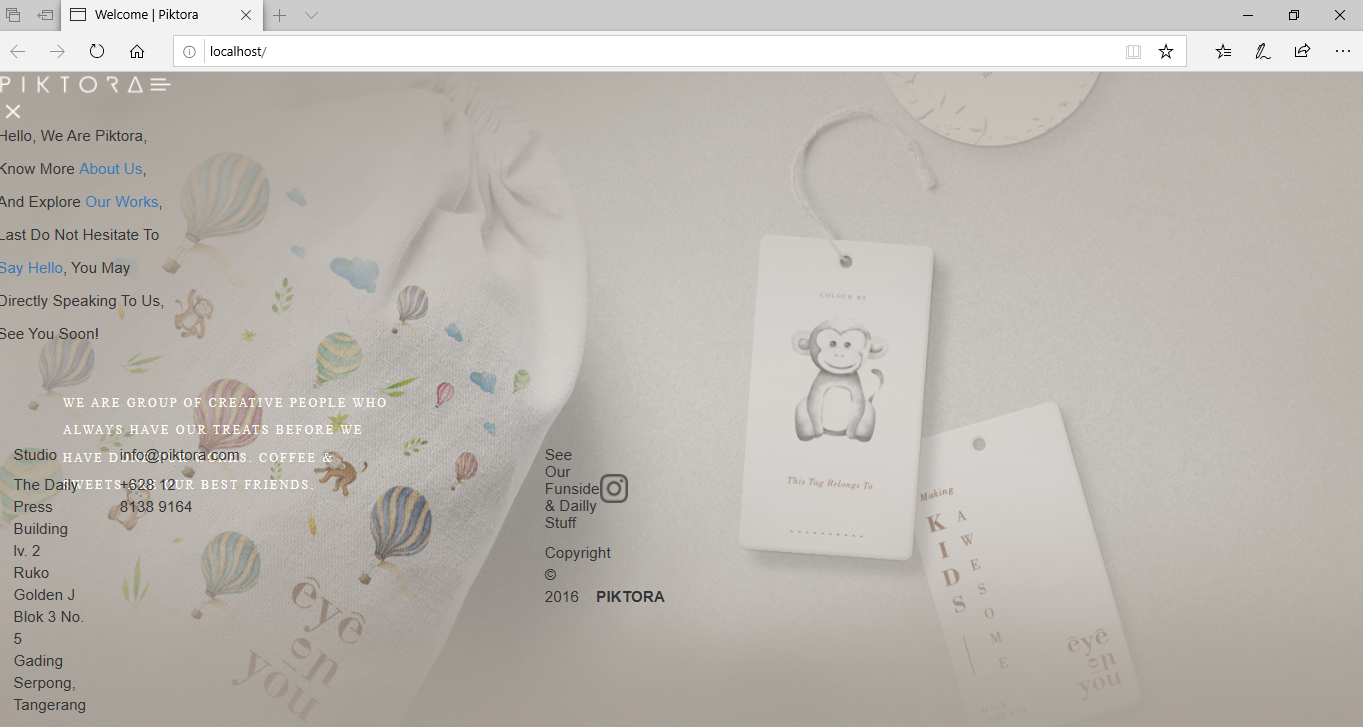
\includegraphics[scale=0.4]{Gambar/Layout_dengan_Edge_Driver.png}
	\caption{Tampilan halaman \textit{web} pada \textit{browser} saat dikontrol oleh EdgeDriver.}
	\label{fig:layout1}
\end{figure}

\begin{figure}[H]
	\centering
		
\includegraphics[scale=0.4]{Gambar/Layout_tanpa_Edge_Driver.png}
	\caption{Tampilan halaman \textit{web} pada \textit{browser} saat tidak dikontrol oleh EdgeDriver.}
	\label{fig:layout2}
\end{figure}
 


\item \textbf{Pengujian Proyek Piktora dengan InternetExplorer}\\
Pengujian pada proyek Piktora dilakukan menggunakan InternetExplorerDriver. Pada saat melakukan pengujian, kode program pada kelas BrowserController baris ke-46  diubah (lihat Lampiran \ref{lamp:A}). \textit{Object} bertipe WebDriver dinisialisasi menggunakan \textit{object} bertipe InternetExplorerDriver. Versi Internet Explorer \textit{browser} yang digunakan untuk pengujian adalah 11.379.17763.0. Gambar \ref{fig:ie_awal} dan Gambar \ref{fig:ie} menunjukkan tampilan pada Internet Explorer \textit{browser} saat sedang dikontrol oleh InternetExplorerDriver. Berikut ini adalah \textit{option} yang digunakan untuk menguji program:
\begin{itemize}
\item \texttt{-project-path C:/xampp/htdocs/Piktora/.git}
\item \texttt{-capture-url http://localhost}
\item \texttt{-before-capture "php script\_piktora.php"}
\end{itemize}
Program berhasil membangkitkan animasi \textit{timelapse} pada proyek Piktora menggunakan InternetExplorerDriver.

\begin{figure}[H]
	\centering
		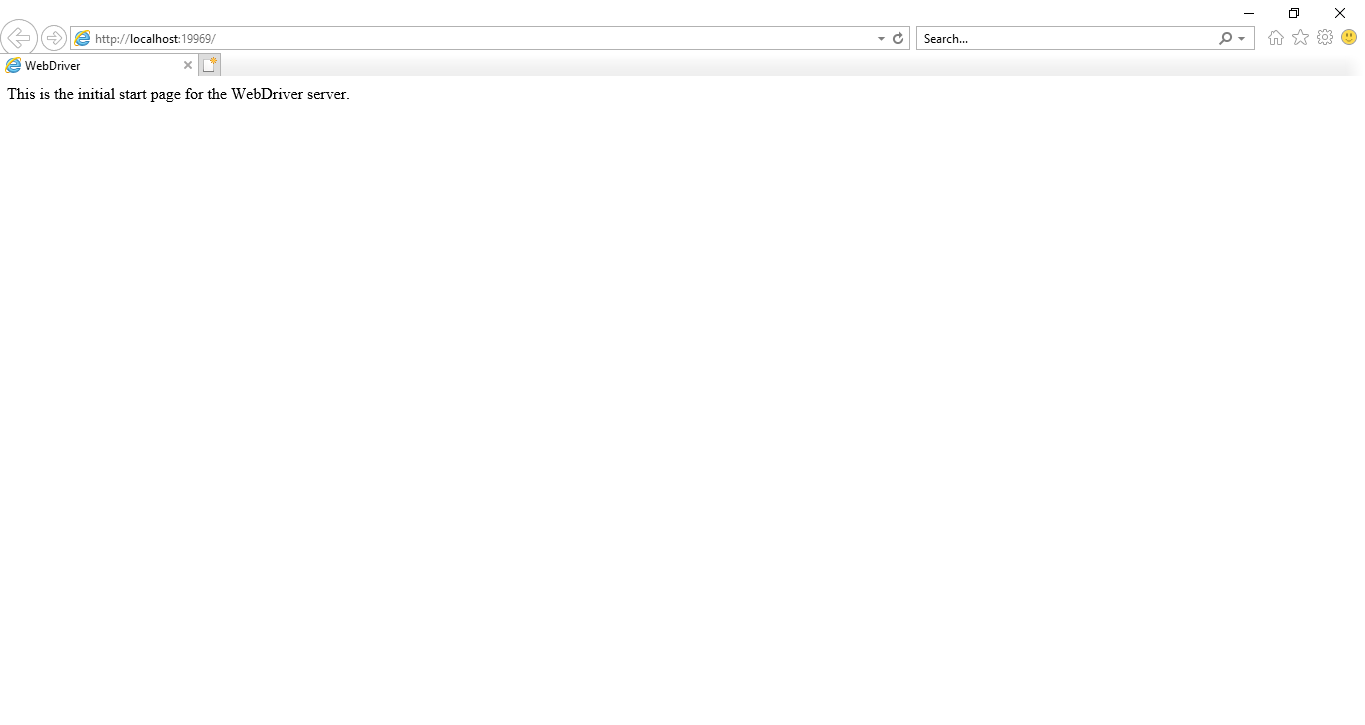
\includegraphics[scale=0.4]{Gambar/IE_awal.png}
	\caption{Keadaan awal dari \textit{browser} saat dikontrol oleh InternetExplorerDriver.}
	\label{fig:ie_awal}
\end{figure}

\begin{figure}[H]
	\centering
		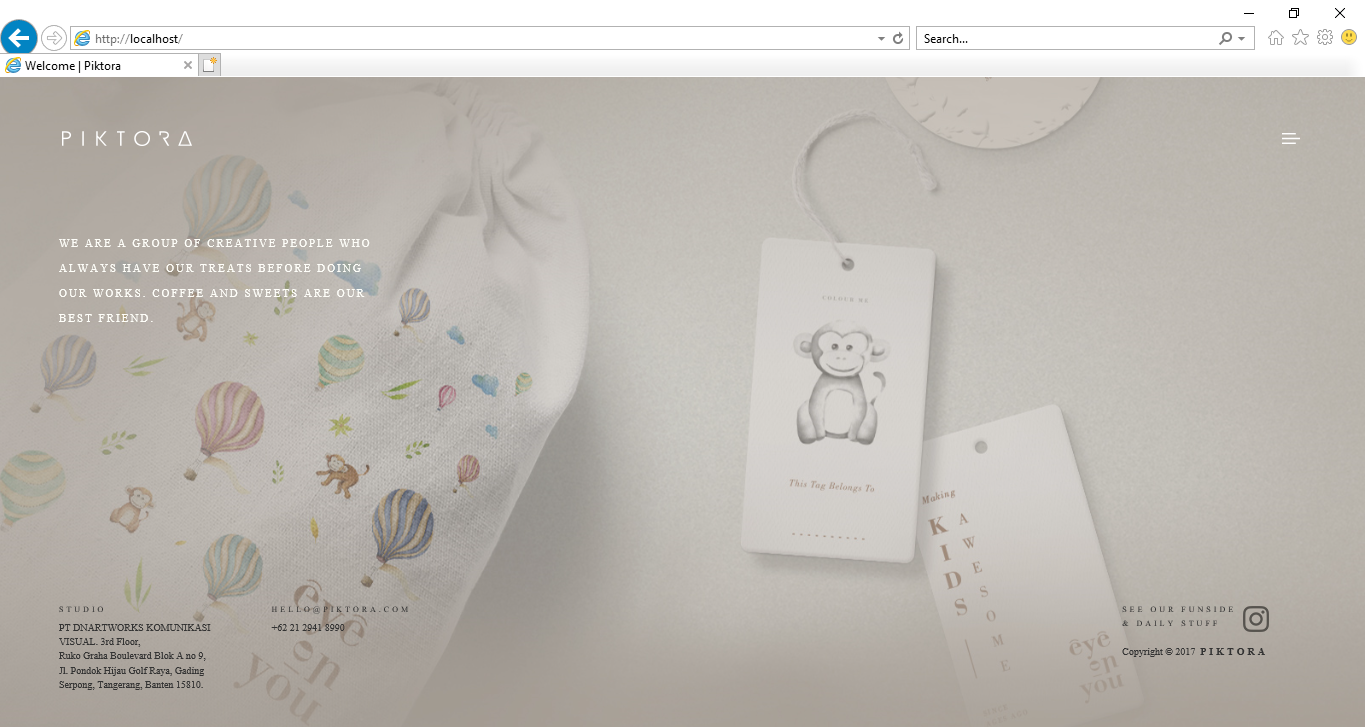
\includegraphics[scale=0.4]{Gambar/IE.png}
	\caption{Tampilan pada \textit{browser} saat dikontrol oleh InternetExplorerDriver. }
	\label{fig:ie}
\end{figure}



\item \textbf{Pengujian Situs \textit{web} Netflix Open Source Software Center}\\
Netflix Open Source Software Center merupakan proyek Open Source yang dimiliki oleh Netflix. Repositori situs \textit{web} ini disimpan pada GitHub\footnote{https://github.com/Netflix/netflix.github.com}. Repositori ini memiliki 393 \textit{commit}. Lingkungan pengujian eksperimental ini sama dengan lingkungan implementasi yang terdapat pada subbab \ref{subsec:lingkunganimplementasi5}. Berikut ini adalah \textit{option} yang digunakan untuk menguji program:
\begin{itemize}
\item \texttt{-project-path C:/xampp/htdocs/netflix.github.com/.git}
\item \texttt{-capture-url http://localhost}
\item \texttt{-seconds-per-commit 0.1} 
\end{itemize}
Program berhasil membangkitkan animasi \textit{timelapse} dari situs \textit{web} Netflix Open Source Software Center. Tidak ditemukan masalah saat melakukan pengujian. Hasil dari pengujian berupa \textit{file} hasil animasi bertipe GIF dengan ukuran 17.5 MB dan berdurasi 39 detik. Sebagian dari hasil animasi dapat dilihat pada Gambar \ref{fig:hasil_netflix}, sedangkan \textit{file} aslinya dapat dilihat pada \textit{link} berikut\footnote{https://github.com/billyAdi/Skripsi/tree/master/Program/TimeLapseGenerator/hasil\%20pengujian/Netflix}.


%Karena \textit{file} hasil animasi bertipe GIF, maka hasilnya tidak bisa ditampilkan pada skripsi ini, tapi bisa dilihat pada link berikut


\begin{figure}[H]	
		\includegraphics[scale=0.3]{Gambar/netflix.jpg}
	\caption{Sebagian hasil animasi dari situs \textit{web} Netflix Open Source Software Center.}
	\label{fig:hasil_netflix}
\end{figure}



\item \textbf{Pengujian Situs \textit{web} Bootstrap}\\
Bootstrap adalah kakas \textit{open source} untuk membangun \textit{website} yang dipakai bersama dengan HTML, CSS, dan JavaScript. Repositori situs \textit{web} ini disimpan pada GitHub\footnote{https://github.com/twbs/bootstrap}. Pengujian ini dilakukan pada \textit{branch} gh-pages, dimana di pada \textit{branch} tersebut terdapat 8547 \textit{commit}. Lingkungan pengujian eksperimental ini sama dengan lingkungan implementasi yang terdapat pada subbab \ref{subsec:lingkunganimplementasi5}. 
Berikut ini adalah \textit{option} yang digunakan untuk menguji program:
\begin{itemize}
\item \texttt{-project-path C:/xampp/htdocs/bootstrap/.git}
\item \texttt{-capture-url http://localhost}
\item \texttt{-seconds-per-commit 0.05} 
\item \texttt{-branch gh-pages}
\end{itemize}

%Terdapat beberapa masalah saat melakukan pengujian situs \textit{web} Bootstrap. Program suatu ketika berhenti dan mengeluarkan pesan error: "short SHA1 685039d is ambiguous". Pesan error ini muncul karena terdapat dua Git \textit{object} yang mempunyai 7 digit ID yang sama, sehingga tidak bisa melakukan \textit{checkout} ke \textit{commit} 685039d. Masalah berikutnya adalah perbedaan letak \textit{file} "index.html". Di beberapa \textit{commit}, \textit{file} "index.html" ini terletak di dalam direktori "docs". Karena perbedaan letak \textit{file} ini, halaman \textit{web} menjadi tidak muncul, yang muncul adalah struktur direktori dari \textit{website} Boostrap. Masalah yang terakhir yaitu di beberapa \textit{commit} tidak terdapat \textit{file} "index.html", sama seperti masalah sebelumnya hal ini menyebabkan halaman \textit{web} menjadi tidak muncul.


Terdapat masalah saat melakukan pengujian situs \textit{web} Bootstrap. Program suatu ketika berhenti dan mengeluarkan pesan error: "short SHA1 685039d is ambiguous". Pesan error ini muncul karena terdapat dua Git \textit{object} yang mempunyai 7 digit ID yang sama, sehingga tidak bisa melakukan \textit{checkout} ke \textit{commit} 685039d. Solusi untuk mengatasi masalah tersebut yaitu dengan mengubah kode program di kelas VCS. Awalnya program hanya menyimpan \textit{commit} ID dengan panjang 7 digit. Setelah itu kode program diubah supaya bisa menyimpan \textit{commit} ID dengan panjang SHA seluruhnya 40 digit.

Pada beberapa \textit{commit}, \textit{file} "index.html" tidak terdapat pada \textit{root directory}. Pada beberapa \textit{commit}, \textit{file} "index.html" terletak pada direktori "docs". Karena tidak terdapat \textit{file} "index.html" halaman \textit{web} menjadi tidak muncul, yang muncul adalah struktur direktori dari repositori Boostrap. 

Setelah itu dilakukan pengujian lagi dengan menggunakan dua argumen pada \texttt{-capture-url}  saat menjalankan program. Setelah menambahkan argumen berupa \texttt{http://localhost/docs} pada \textit{option} \texttt{-capture-url} dan mengubah kode program di kelas VCS, program berhasil membangkitkan animasi. Hasil dari pengujian berupa \textit{file} hasil animasi bertipe GIF dengan ukuran 160 MB dan berdurasi 7 menit 7 detik. Sebagian dari hasil animasi dapat dilihat pada Gambar \ref{fig:hasil_bootstrap}.


\begin{figure}[H]	
		\includegraphics[scale=0.3]{Gambar/Bootstrap.jpg}
	\caption{Sebagian hasil animasi dari situs \textit{web} Bootstrap.}
	\label{fig:hasil_bootstrap}
\end{figure}



%Karena \textit{file} hasil animasi bertipe GIF, maka hasilnya tidak bisa ditampilkan pada skripsi ini.




%Solusi untuk mengatasi masalah pertama yaitu dengan mengubah kode program di kelas VCS. Awalnya program hanya menyimpan \textit{commit} ID dengan panjang 7 digit. Setelah itu kode program diubah supaya bisa menyimpan \textit{commit} ID dengan panjang 40 digit. 

%Solusi untuk mengatasi masalah kedua yaitu dengan menambahkan \textit{Option} \texttt{-before-capture} saat menjalankan program. Argumen dari Option tersebut berisi \textit{terminal command} yang menjalankan \textit{script} PHP. \textit{Script} PHP ini akan mengecek letak \textit{file} "index.html" pada \textit{folder} utama dan "docs". \textit{Script} kemudian akan mengecek \textit{directory root} apache pada \textit{file} "httpd.conf". Jika \textit{directory root} sudah mengarah ke \textit{folder} tempat "index.html" berada, maka \textit{script} tidak akan mengubah isi \textit{file} "httpd.conf". Jika \textit{directory root} tidak mengarah ke \textit{folder} tempat "index.html" berada, maka \textit{script} akan mengubah \textit{directory root} pada \textit{file} "httpd.conf" dan melakukan \textit{restart} pada apache.

%Untuk masalah ketiga, belum ditemukan solusinya. Jadi program akan tetap mengambil \textit{screenshot} meskipun tidak terdapat \textit{file} "index.html". Setelah menambahkan \textit{Option} \texttt{-before-capture} dan mengubah kode program sehingga menyimpan \textit{commit} ID dengan panjang 10 digit, program berhasil membangkitkan animasi. Hasil dari pengujian berupa \textit{file} hasil animasi bertipe GIF dengan ukuran 281 MB dan berdurasi 7 menit 7 detik. Karena \textit{file} hasil animasi bertipe GIF, maka hasilnya tidak bisa ditampilkan pada skripsi ini.

\item \textbf{Pengujian Situs \textit{web} IBM Open Source}\\
IBM Open Source merupakan proyek Open Source yang dimiliki oleh IBM. Repositori situs \textit{web} ini disimpan pada GitHub\footnote{https://github.com/IBM/ibm.github.io}. Repositori ini memiliki 263 \textit{commit}. Lingkungan pengujian eksperimental ini sama dengan lingkungan implementasi yang terdapat pada subbab \ref{subsec:lingkunganimplementasi5}. Berikut ini adalah \textit{option} yang digunakan untuk menguji program:
\begin{itemize}
\item \texttt{-project-path C:/xampp/htdocs/ibm.github.io/.git}
\item \texttt{-capture-url http://localhost}
\item \texttt{-seconds-per-commit 0.1} 
\end{itemize}
Program berhasil membangkitkan animasi \textit{timelapse} dari situs \textit{web} IBM Open Source. Tidak ditemukan masalah saat melakukan pengujian. Hasil dari pengujian berupa \textit{file} hasil animasi bertipe GIF dengan ukuran 15.2 MB dan berdurasi 26 detik. Sebagian dari hasil animasi dapat dilihat pada Gambar \ref{fig:hasil_ibm}, sedangkan \textit{file} aslinya dapat dilihat pada \textit{link} berikut\footnote{https://github.com/billyAdi/Skripsi/tree/master/Program/TimeLapseGenerator/hasil\%20pengujian/IBM}.


%Karena \textit{file} hasil animasi bertipe GIF, maka hasilnya tidak bisa ditampilkan pada skripsi ini, tapi bisa dilihat pada link berikut\footnote{https://github.com/billyAdi/Skripsi/tree/master/Program/TimeLapseGenerator/hasil\%20pengujian/IBM}.

\begin{figure}[H]	
		\includegraphics[scale=0.3]{Gambar/ibm.jpg}
	\caption{Sebagian hasil animasi dari situs \textit{web} IBM Open Source.}
	\label{fig:hasil_ibm}
\end{figure}


\item \textbf{Pengujian Situs \textit{web} React}\\
React merupakan \texttt{library} Java Script yang digunakan untuk membangun antarmuka. Repositori situs \textit{web} ini disimpan pada GitHub\footnote{https://github.com/facebook/react}. Repositori ini memiliki 570 \textit{commit}. Lingkungan pengujian eksperimental ini sama dengan lingkungan implementasi yang terdapat pada subbab \ref{subsec:lingkunganimplementasi5}. Berikut ini adalah \textit{option} yang digunakan untuk menguji program:
\begin{itemize}
\item \texttt{-project-path C:/xampp/htdocs/react/.git}
\item \texttt{-capture-url http://localhost}
\item \texttt{-seconds-per-commit 0.05}
\item \texttt{-branch gh-pages} 
\end{itemize}
Program berhasil membangkitkan animasi \textit{timelapse} dari situs \textit{web} React. Untuk beberapa \textit{commit} tidak terdapat \textit{file} "index.html". Hasil dari pengujian berupa \textit{file} hasil animasi bertipe GIF dengan ukuran 18.2 MB dan berdurasi 28 detik. Sebagian dari hasil animasi dapat dilihat pada Gambar \ref{fig:hasil_react}, sedangkan \textit{file} aslinya dapat dilihat pada \textit{link} berikut\footnote{https://github.com/billyAdi/Skripsi/tree/master/Program/TimeLapseGenerator/hasil\%20pengujian/React}.


\begin{figure}[H]	
		\includegraphics[scale=0.3]{Gambar/react.jpg}
	\caption{Sebagian hasil animasi dari situs \textit{web} React.}
	\label{fig:hasil_react}
\end{figure}


%Karena \textit{file} hasil animasi bertipe GIF, maka hasilnya tidak bisa ditampilkan pada skripsi ini, tapi bisa dilihat pada link berikut\footnote{https://github.com/billyAdi/Skripsi/tree/master/Program/TimeLapseGenerator/hasil\%20pengujian/React}.


\item \textbf{Pengujian Situs \textit{web} Yelp Open Source}\\
Yelp Open Source merupakan proyek Open Source yang dimiliki oleh Yelp. Repositori situs \textit{web} ini disimpan pada GitHub\footnote{https://github.com/Yelp/yelp.github.io}. Repositori ini memiliki 99 \textit{commit}. Lingkungan pengujian eksperimental ini sama dengan lingkungan implementasi yang terdapat pada subbab \ref{subsec:lingkunganimplementasi5}. Berikut ini adalah \textit{option} yang digunakan untuk menguji program:
\begin{itemize}
\item \texttt{-project-path C:/xampp/htdocs/yelp.github.io/.git}
\item \texttt{-capture-url http://localhost}
\item \texttt{-seconds-per-commit 0.2} 
\end{itemize}
Program berhasil membangkitkan animasi \textit{timelapse} dari situs \textit{web} Yelp. Tidak ditemukan masalah saat melakukan pengujian. Hasil dari pengujian berupa \textit{file} hasil animasi bertipe GIF dengan ukuran 4.63 MB dan berdurasi 19 detik. Sebagian dari hasil animasi dapat dilihat pada Gambar \ref{fig:hasil_yelp} , sedangkan \textit{file} aslinya dapat dilihat pada \textit{link} berikut\footnote{https://github.com/billyAdi/Skripsi/tree/master/Program/TimeLapseGenerator/hasil\%20pengujian/Yelp}.


\begin{figure}[H]	
		\includegraphics[scale=0.3]{Gambar/yelp.jpg}
	\caption{Sebagian hasil animasi dari situs \textit{web} Yelp.}
	\label{fig:hasil_yelp}
\end{figure}



%Karena \textit{file} hasil animasi bertipe GIF, maka hasilnya tidak bisa ditampilkan pada skripsi ini, tapi bisa dilihat pada link berikut\footnote{https://github.com/billyAdi/Skripsi/tree/master/Program/TimeLapseGenerator/hasil\%20pengujian/Yelp}.

\end{enumerate}




\begin{table}[htbp]
	\centering
	\caption{Tabel hasil pengujian eksperimental menggunakan beberapa situs \textit{web}}
	
		\begin{tabular}{|p{0.3cm}| p{5 cm}| p{3 cm }|p{3 cm}| p{3 cm}|} \hline
		No & Situs \textit{web}	& Jumlah \textit{commit} &Ukuran \textit{output file}  & Durasi animasi \\ \hline
		1. & Yelp Open Source & 99 &4.63 MB  & 19 detik\\ \hline
		2. & IBM Open Source & 263&15.2 MB  & 26 detik	\\ \hline	
		3. & Netflix Open Source Software Center & 393 &17.5 MB & 39 detik  \\ \hline
		4. & React & 570 & 18.2 MB  & 28 detik \\ \hline
		5. & Bootstrap & 8547 &160 MB & 7 menit 7 detik  \\ \hline
		\end{tabular}
	\label{table:hasil_eksperimental}
\end{table}

Tabel \ref{table:hasil_eksperimental} merupakan rekap dari hasil pengujian experimental menggunakan beberapa situs \textit{web}. Pada Tabel \ref{table:hasil_eksperimental} dapat dilihat hubungan antara ukuran \textit{output file} dengan jumlah \textit{commit}. Dapat dilihat bahwa semakin besar jumlah \textit{commit}, ukuran \textit{file} yang dihasilkan semakin besar.

Hal yang menarik dari pengujian eksperimental adalah letak \textit{file} "index.html" yang tidak konsisten pada repositori situs \textit{web} Bootstrap. Pada beberapa \textit{commit}, \textit{file} "index.html" berada pada \textit{root directory}. Pada beberapa \textit{commit}, \textit{file} "index.html" berada pada direktori "docs". Pada beberapa \textit{commit} tidak terdapat \textit{file} "index.html". Pada beberapa \textit{commit} terakhir, saat membuka \textit{file} "index.html" pada direktori "docs", halaman menjadi dialihkan ke situs \textit{web} Bootstrap\footnote{https://getbootstrap.com/docs/4.3/getting-started/introduction}.


Berdasarkan hasil pengujian eksperimental, didapatkan kesimpulan sebagai berikut:
\begin{enumerate}
\item Semakin besar jumlah \textit{commit} pada repository semakin besar ukuran \textit{file} yang dihasilkan.
\item Untuk repositori situs \textit{web} yang sederhana seperti Netflix Open Source Center, Bootstrap, IBM Open Source, React, dan Yelp Open Source, tidak dibutuhkan \textit{option} \texttt{-before-capture} untuk membangkitkan animasi. Untuk repositori yang memerlukan setup basis data seperti Piktora, dibutuhkan \textit{option} \texttt{-before-capture} untuk membangkitkan animasi. 
\item Program dapat membangkitkan animasi dengan baik saat menggunakan OperaDriver, FirefoxDriver, dan InternetExplorerDriver. Saat dilakukan pengujian menggunakan EdgeDriver, tampilan dari halaman \textit{web} menjadi tidak rapih.
\end{enumerate}

